\documentclass[14pt]{article}
%\documentclass[14pt]{llncs}
\usepackage[left=2.5cm,right=2.5cm,top=2.5cm,bottom=2.5cm]{geometry}
%\usepackage[a4paper, total={6in, 8in}]{geometry}
\usepackage{amsmath,amssymb,amsfonts} % mathematical and other 
% special symbols and fonts
\usepackage{tikz} % support for drawing graphs and diagrams
\usetikzlibrary{arrows,decorations.pathmorphing,positioning,fit}
\usetikzlibrary{trees,shapes}
\usepackage[pdfpagelabels=true,linktocpage]{hyperref} % hyperlink 
% support (also internal links)
\usepackage{xcolor} % color support
\usepackage{listings} % listings and \lstinline support for code 
% typesetting
\lstset{language=C++}
\usepackage[english]{babel} % needed for English texts (translations, 
% e.g. References --> Literatur)
% \usepackage[ngerman]{babel} % needed for German texts (translations, 
%e.g. References --> Literatur)
\usepackage[utf8]{inputenc} % unicode encoding
\usepackage{graphicx} % support for \includegraphics{}
\usepackage{float}
\usepackage{enumerate} % support of different styles of enumerations
%\usepackage[section]{algorithm}
\usepackage{newalg}
\usepackage{paralist}

\usepackage{url}
\usepackage{qtree}

\usepackage{tikz}
\usetikzlibrary{trees}

\usepackage{tikz}
\usetikzlibrary{shapes}
\usepackage{amsmath}
\usepackage{xspace}
\newcommand{\A}{\ensuremath{\mathcal{A}}\xspace}
\newcommand{\B}{\ensuremath{\mathcal{B}}\xspace}
\newcommand\pa[1]{\ensuremath{\left(#1\right)}}


\usepackage{dot2texi} 



\usepackage[listings,theorems]{tcolorbox}
\tcbset{before={\par\medskip\pagebreak[0]\noindent},after={\par\medskip}}%

\usepackage{amsmath}
\usepackage{booktabs}
\usepackage{caption}

%\captionsetup[table]{position=top}


% By default the URLs are put in typewriter type in the body and the
% bibliography of the document when using the \url command.  If you are
% using many long URLs you may want to uncommennt the next line so they
% are typeset a little smaller.
\renewcommand{\UrlFont}{\small\tt}


\newtheorem{definition}{Definition}[section] % defines the definition environment
\newtheorem{theorem}{Theorem}[section] % defines the theorem environment
\newtheorem{proof}{Proof}[section] % defines the proof environment
\newtheorem{Algorithm}{Algorithm} % defines the algorithm environment

%\floatstyle{boxed}		% Puts a figure
%\restylefloat{figure}	% into a box.
\floatstyle{ruled}					% Puts an algorithm
\newfloat{Algorithm}{thp}{lop}		% between a head and
\floatname{Algorithm}{Algorithm}	% a foot line
\restylefloat{table}	% Puts a table between a head and a foot line



%Define often used expressions:
\newcommand{\True}{\ensuremath{\textit{True}~}}
\newcommand{\False}{\ensuremath{\textit{False}~}}
\newcommand{\TikZ}{Ti\emph{k}Z}

\newcommand{\rom}[1]{\uppercase\expandafter{\romannumeral #1\relax}}
%\renewcommand{\baselinestretch}{1.3}

% A nice opportunity to comment the text is given by the following:
%\usepackage{todonotes}
%\definecolor{lightgreen}{rgb}{0.8,1.0,0.8}
%\definecolor{lightblue}{rgb}{0.8,0.85,1}
%\newcommand{\Author}[1]{\todo[inline,color=lightgreen]{A: #1}}
%\newcommand{\Supervisor}[1]{\todo[inline,color=lightblue]{S: #1}}


\title{SMT for Strings \\ {\large Seminar:
		Satisfiability Checking} \\ {\large SS 2015}}
\author{Meshkatul Anwer \\ Supervision: Cornelius Aschermann}
%\institute{ RWTH Aachen}


\begin{document}
	
	\maketitle
	
    \begin{abstract}
Our modern society relies on software systems and on-line services. Most of the times these systems are dealing with our private and sensitive data. Privacy violation is one of the major concerns about such web-based applications and on-line services. To provide a more secure environment for the Internet services, these web-based applications should be tested for vulnerability. The verification procedure and security analysis of such system rely on automatic solvers, which can check the satisfiability of constraints over a rich set of data types, including character strings. String is considered as the main information carrier in web-based communication. However, most traditional mathematical methods focus more on numbers and most string solvers today are standalone tools that can reason only about some fragment of the theory of strings. In this paper we will describe a solver for the theory of unbounded strings with concatenation and length. 
\end{abstract}
	\section{Introduction}
\label{sec:introduction}
Stability and reliability of software systems has been a key issues in the protection of privacy and security. As we want more and more new features and functionalists into such systems, the complexity of the system is exploding. With the rise of web-based applications and online services, the amount of information sharing via networking has increased rapidly. As a result, the security of web applications is getting more and more attention. As the complexity of such systems is growing, manual analysis is getting harder and sometime impossible.  In the last few years, a number of techniques which were originally developed for automatic verification purposes have been adopted for the software security analysis. 

The ability to reason about string values is a major task in the field of security analysis. Especially in web-based applications, where the program inputs are often provided as strings. These strings are usually get processed through operations such as matching against regular expressions, concatenation, and substring extraction or replacement. We need to be able to formally reason about strings as well as other data types.  


In this paper, we will see how the automatic reasoning engines such as Satisfiability Module Theories (SMT) solvers, are helping to check the satisfiability of constraints over rich set of data types including  strings. We will describe a  SMT solver for strings. The ideas are presented in paper \cite{main-paper} and a practical version of the solver is implemented into the SMT solver CVC4 \cite{cvc4_website} core.
	%\section{Motivating Example}
We are interested in SMT solver which helps to check the satisfiability of constraints over rich set of data types. Here we will see few examples such constraints on strings. Example 3 shows how we can express regular expression membership constraint.

\begin{description}
\item[Example  1: ] Find an assignment for \(x\), where \(x."ab"="ba".x \wedge  len(x) =7\).
\item[Example  2: ] Find a model for \(x\), \(y\) and \(z\), where \(x."ab".y=y."ba".z \wedge z=x.y \wedge x."a" \neq "a".x\).
\item[Example  3: ] Find a model for \(x\) and \(y\), where both \(x\) and \(y\) are in the \(RegEx (a*b)*\) and they are different but have the same length.
\end{description}
Where \(x\), \(y\) and \(z\) are variables of type string, \(len\) is a function which returns the length of the string variable.  Figure \ref{fig:smt_example_1_2} and \ref{fig:smt_example_3} show the encoding of Example 1 , Example 2 and Example 3 in smt-lib \cite{smtlib:website} format. The examples and code snippets  are taken from \cite{cvc4:wiki}.

\begin{figure}[ht]
	\centering
	\begin{minipage}[t]{0.45\linewidth}
		\begin{verbatim}
		...		
		(assert (= (str.++ x "ab") (str.++ "ba" x)))
		(assert (= (str.len x) 7))
		
		...
		\end{verbatim}
	\end{minipage}
	\quad
	\begin{minipage}[t]{0.45\linewidth}
		\begin{verbatim}
		...
		(assert (= (str.++ x "ab" y) (str.++ y "ba" z)))
		(assert (= z (str.++ x y)))
		(assert (not (= (str.++ x "a") (str.++ "a" x))))
		...
		\end{verbatim}
	\end{minipage}
	\caption{Encoding of Example 1 and Example 2 in smt-lib \cite{smtlib:website} format.}
	\label{fig:smt_example_1_2}
\end{figure}
\begin{figure}[ht]
	\centering
    \begin{minipage}[t]{0.65\linewidth}
		\begin{verbatim}
		...
		(assert(str.in.re x(re.* (re.++ (re.* (str.to.re "a") ) (str.to.re "b") ))))
		(assert (str.in.re y(re.* (re.++ (re.* (str.to.re "a") ) (str.to.re "b") ))))
		
		(assert (not (= x y)))
		(assert (= (str.len x) (str.len y)))
		...
		\end{verbatim}
	\end{minipage}
	\caption{Encoding of Example 3 in smt-lib \cite{smtlib:website} format.}
	\label{fig:smt_example_3}
\end{figure}

In the context of security analysis, modern SMT solver is used as the core constraint solver. The idea is to reduce security problems to constraint satisfaction problems in some formal logic. If the constraints are unsatisfiable, the source code is free of any exploit; otherwise, there is an assignment (of variables in the constraints) that satisfies these constraints and defines a possible attack. Traditionally analysis tools use their own built-in constraint solvers. However, it is possible to encode a security analysis problem into a Satisfiability Modulo Theories (SMT) problem. Then the preexisting standard SMT solver, which combines a SAT solver with multiple specialized theory solvers can be used. As string is the dominant data type in modern web-applications, constraints over strings along with other data types need to be checked. In this paper we will have a look into a string solver.
	\section{Security analysis with theory solvers}
In the context of security analysis, we want to find out whether security flaws exist in a piece of program. To answer such questions, we express security specification and properties as a set constraints in some background theories. Then this set of constraints is provided to an automatic reasoning tool, which should answer whether the constraints are satisfiable or not. The usual intension is to get the bug revealing inputs reported by the tool. The conventional manual testing or verification processes may not be compete. As they usually model partial scenarios. Whereas the automatic reasoning tool facilitates the search of whole space for possible flaws. Thats why the approach of verification with the help SMT solvers is quite reliable, efficient and complete.

	\begin{description}
		\item[Example:] Here is an example of such constraint,
		\begin{equation}
		\label{mainConstraint}
		assert (x =  \texttt{con}("ab", z) \wedge (y =  \texttt{con}("de", z) \vee y =  \texttt{con}("abc", l) ) \wedge x =  y \wedge \texttt{len} (x) > 6)
		\end{equation}
		where \texttt{con} and \texttt{len} are functions with the usual meaning of string concatenation function and string length function and $x, y, z$ and $l$ are variables of type string. Figure \ref{figure:main-formula-smtlib} shows how this formula can be encoded into the language of theory solver. 
	\end{description}
	
	\begin{figure}[width=4cm]
		\scriptsize
		\centering
		\begin{lstlisting}
		(set-option:produce-models true)
		(set-logic QF_S)
		
		(declare-fun x () String)
		(declare-fun y () String)
		(declare-fun z () String)
		(declare-fun l () String)
		
		(assert (= x (str.++ "ab" z)))
		(assert (or (= y (str.++ "de" z)) (= y (str.++ "abc" l))) )
		(assert (=  x  y)) 
		(assert (> (str.len x) 6)) 
		
		(check-sat)
		(get-value (x y z l) )	
		\end{lstlisting}
		\caption{ \scriptsize The formula \ref{mainConstraint} is encoded into smt-lib\cite{smtlib:website} format.}
		\label{figure:main-formula-smtlib}
	\end{figure}
	When this constraint is provided to the theory solver and asked for satisfiability check, it answers with a satisfying solution like,	
	\[
	x = "abcAAAA", \ y ="abcAAAA", \ z = "cAAAA" \textnormal{and} \ l = "AAAA" 
	\]
	The example shows how complex constraints can be expressed. Especially in the context of security analysis we want to express complex constrains over strings and other data types. The ability to reason over strings and other data types is very important. Many security analysis tools exists in the industry and used for practice. However, they are either able to reason on certain theories or they are very limited in expressiveness. In this paper, we will present a general purpose theory solver for strings and length constraints.	
	\section{Related work}
\label{sec:Related work}

There has been a lot of research effort on the development of the efficient theory solver for Strings \cite{misc_89}. Theoretically the general world equation problem or the satisfiability problem of theory of strings(with most of common string functions) is undecidable \cite{misc_17}. However, a restricted theories of strings is decidable and practically useful. Different approaches to solve the problem have been proposed and implemented. A class of solvers is based on reducing the string constraints to constraints in other theories e.g. theory of bit-vector. Examples of such solver are Hampi \cite{hampi} and Kaluza \cite{Kaluza}. However, they can only solve problem over fixed length strings. 

In this paper, we will present a SMT solver for strings based an algebraic approach. The whole decision procedure is described as a set of derivation rules and their application strategy. The procedure allows to express the constraints over unbounded strings. A practical theory solver over string based on this approach has been implemented into the CVC4 SMT solver\cite{cvc4_website} core. The detail of the description can be found in the paper \cite{main-paper}. We will try to explain the main ideas presented by the authors.    
	
\section{Background}
\label{sec:Background}

In this section, we will present an introduction over the SMT problem solving. Later we will focus on the theory solver part.

\subsection{The SAT problem}
In classical propositional logic, a boolean formula is constructed from a set of variables connected by logical operators like \(\wedge, \vee, \neg\). The boolean variables can be assigned a truth value that is either  $\texttt{true}$ or  $\texttt{false}$. The classical $ SAT\ problem$is defined as, 
given a boolean formula, is there any assignment, such that the formula is evaluated to $\texttt{true}$. There are many decision procedures to solve this classic SAT problem. Among them, the DPLL \cite{dpll} procedure is  most frequently used in most modern SAT solvers. 

\subsection{The SMT Problem}
\label{sec:dpllt procedure}
The DPLL procedure takes a set of clauses as input. It returns $\texttt{sat}$ if a logically consistent assignment can be found; otherwise, it returns $\texttt{unsat}$. For example, 
\[
	s_1 \wedge (s_2 \vee s_3) \wedge s_4 \wedge s_5
\] 
	is a boolean formula for the example \ref{mainConstraint}. Where each $s_i$ is  just a representation for each constraint. The DPLL procedure does not need to interpreted the actual meaning of the constraint. When the set $ \{ s_1, s_2 \vee s_3, s_4, s_5 \}$ is given as input, the DPLL procedure returns partial assignment. 
	
	\[
		\{ s_1 ,\ (s_2 \vee s_3),\ s_4, \ s_5 \} \mapsto \{ s_1 ,\ s_2 ,\ s_4, \ s_5 \}\  \textnormal{or}\ \{ s_1 ,\ s_3 ,\ s_4, \ s_5 \} 
	\]
	Now this partial assignments are need to be checked for satisfiability. Each boolean variable in the partial assignments represents a constraint. The constraints may have function symbols (e.g. \texttt{con}, \texttt{len}) or predicate symbols. The meaning of the variables, constants, predicates and functions must be defined. In SMT formulas, the signature is extended to a set of predicate symbols, a set of function symbols and a set of non-boolean variables. Those extended symbols can only be interpreted in some background theories. We say an SMT formula is satisfiable if there exists a model that satisfies both the logical formula and the background theories. In our case the relevant background theories are  $\mathcal{T}_{SL}$ and $\mathcal{T}_{LIA}$. We are focusing on the solver for the theory $\mathcal{T}_{SL}$. We will use $\mathcal{T}_{SL}$-solver to denote the theory solver for strings.

\begin{figure}[htb]
	\begin{center}
		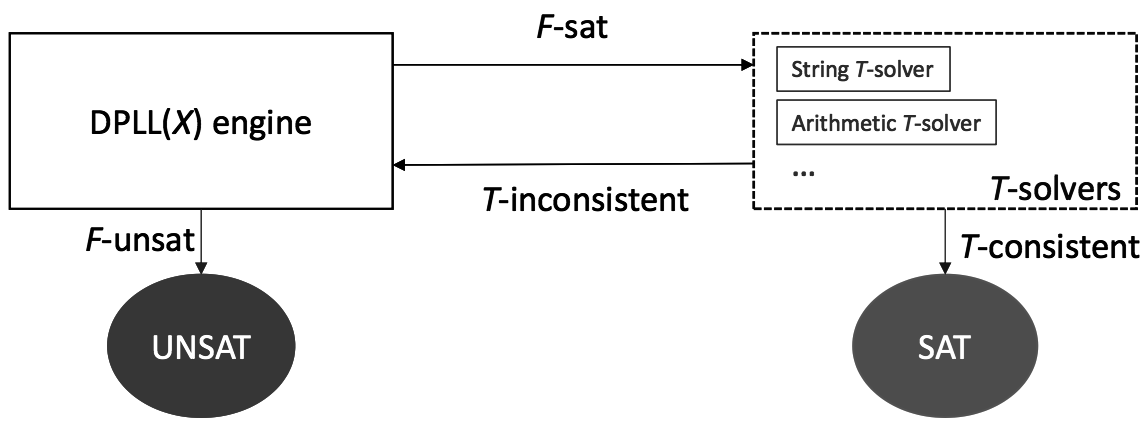
\includegraphics[width=0.8\linewidth]{pictures/dpll_arc.png}
	\end{center}
	\caption{An overview of the interaction between SAT core and $\mathcal{T}$-solvers. The image is sourced from \cite{main_phd}.}
	\label{fig:dpll_architecture}
\end{figure}

The SMT problem solving procedure  can be divided into two parts, as shown in Figure \ref{fig:dpll_architecture} : the logic solving part and the theory solving part. In the logic solving part, it usually refers to the DPLL-based SAT solver with  the capability to handle incremental clause assertions. The theory solving part usually contains several dedicated solvers for background theories. 

Initially, the SAT solver gets the formula as input. It tries to find a model for the literals. If fails, it returns $\texttt{unsat}$; otherwise, it distributes each literal to a corresponding $\mathcal{T}$-solver according to the signature of the literal.

When a $\mathcal{T}$-solver gets a set of literals, it first checks whether these literals are consistent with the theory. If it is $\mathcal{T}$-consistent, the $\mathcal{T}$-solver does nothing but reports consistent back to the SAT core. Otherwise, it either returns a conflict, or propagates a new literal. For example,  in case of our example, when the partial model $\{ s_1 ,\ s_2 ,\ s_4, \ s_5 \}$ is given to the $\mathcal{T}_{SL}$-solver. It finds a  contraction $s_1 \wedge s_2 \to \neg s_4$ and reports back to the core. 

If all $\mathcal{T}$-solvers report $\mathcal{T}$-consistent, the procedure stops and answers $\texttt{sat}$ with the current partial assignments as model ; otherwise, the SAT solver collects all clauses returned by $\mathcal{T}$-solvers, and asserts them into the formula. Then, it tries to build a model from this new formula. For example,  in case of our example, the core add $\neg s_2$ as a new fact and starts over again.	
    \section{The Theory Solver}
\label{sec:the theory solver}
In this section we will focus on the SMT solver for strings, which can handle a finite set of (unbounded)string constraints and length constraints.

\subsection{Core Language}
\label{sec:Core language}
We use \( \Sigma_{SL}\) to denote the signature over the String sort and the Integer sort. 
The common symbols (e.g., \( + , - ,  \le \) ) of linear integer arithmetic are interpreted with their usual meaning. The signature defines a finite set of alphabets $\mathcal{A}$ (e.g. 256 ascii characters). A valid string will have characters only from  $\mathcal{A}$. The terms of sort string can be :
\begin{description}
	\item[-] constants symbol e.g. $'a', 'ab', 'abc','helloworld'$. That is any word from  $\mathcal{A}^*$. 
    \item[-] variables symbol e.g. $x, y, z$.
	\item[-] function symbol \($\underline{con}$ : String \times \cdots \times String \to String\), interpreted as the word concatenation;
	\item[-] a function symbol \($\underline{len}$ : String  \to Int \), interpreted as the word length function;    
\end{description}
We have two types of constraints depending on the signature:
\begin{description}
	\item[-] \( string \ constraint \) : is a (dis)equality  \( (\neg) s \approx t \) with \(s\) and \(t\) are string terms; e.g.
		     $x =  \texttt{con}("ab", z) $,
	         $y =  \texttt{con}("de", z) $,  
	         $y =  \texttt{con}("abc", l)$,  
	         $x =  y$.   
    \item[-] \( length \ constraint \) : is a (dis)equality  \( (\neg) s \approx t \) or \( (\neg) s > t \) where \(s\) and \(t\) are arithmetic terms; e.g. $\texttt{len}\ x > 6$.
\end{description}
Throughout the section we will use $S$ to denote the set of constraints over strings terms and $A$ to denote set of arithmetic constraints. For example, 
\[
S = \{      x =  \texttt{con}("ab", z) ,y =  \texttt{con}("abc", l),x =  y. \},
A = \{      \texttt{len}\ x > 6. \}
\]
where, $x,y,z,l$ are variables of type string. If \(x\) and \(y\) are string variables, \(\texttt{len} \ x\) is both a string and an arithmetic term and  \((\neg)\texttt{len} \ x \approx \texttt{len} \ y\) is both a string and an arithmetic constraint. A \(\mathcal{T}_{SL}\)-constraint is a string, arithmetic constraint. We will use \( \models_{SL}\) to denote entailment in \(\mathcal{T}_{SL}\).
      \subsection{The decision procedure}  
  The decision procedure is defined as a set of derivation rules. The procedure starts with an initial configuration keeps applying the derivation rules according to the strategy. During this repeated application of rules a derivation tree is produced.  When any rule is selected for application, it may cause the tree to branch at this configuration. These  rules are usually called spiting rules. A configuration may be \texttt{unsat}. If the procedure reaches a configuration which is \texttt{unsat}, it will backtrack and choose another branch for rule application. If there is no other branch in case of \texttt{unsat}, we call the branch is closed. Another possibility is that, the procedure reaches a configuration, where no more rule application is possible. Such a configuration is a $staturated$ one. A derivation tree is called $closed$ if all of its branches are closed. If the procedure ends up with a closed derivation tree, it concludes that the set of constraints are unsatisfiable or declares \texttt{unsat}. On the other hand,  If the procedure ends up with a saturated configuration, it concludes that the set of constraints are satisfiable or declares \texttt{unsat}. Whenever any new string constraint is derived from any rule application, the procedure restart. 
      
  At the start of the procedure, each term in the set of constraints must be in their normalized form according to the reduction rules listed below.   

					  \begin{align*}
					  \texttt{con}(\mathbf{s},  \texttt{con}(\mathbf{t}), \mathbf{u}) &\rightarrow   \texttt{con}(\mathbf{s},\mathbf{t}, \mathbf{u})\\
					  \texttt{con}(\mathbf{s}, \epsilon, \mathbf{u}) &\rightarrow \texttt{con}(\mathbf{s}, \mathbf{u})\\
					  \texttt{con}(s) &\rightarrow s\\
					  \texttt{con}() &\rightarrow \epsilon\\
					  \texttt{con}(\mathbf{s}, c_1 \cdots c_i, c_{i+1} \cdots c_n, \mathbf{u}) &\rightarrow \texttt{con}(\mathbf{s}, c_1 \cdots c_n, \mathbf{u})\\
					  \texttt{len}( \texttt{con}(s_1,\cdots,s_n)) &\rightarrow \texttt{len}(s_1) + \cdots + \texttt{len}(s_n)\\
					  \texttt{len}(c_1,\cdots,c_n) &\rightarrow n
					  \end{align*}					 
  Here is few examples of terms and their normal forms, 
  $\texttt{con}("ab", \texttt{con}("c", l)) \rightarrow \texttt{con}("abc",l) $, $\texttt{len}("abc") \rightarrow 3$,\\ $\texttt{len}(\texttt{con}("abc", "def"))\rightarrow 6$. 
  
  
  The procedure starts applying rules on the initial configuration according to the following steps:
  \begin{enumerate}   
    \item $Check\ conflicts:$ The idea is to drive conflict as early as possible. Apply \texttt{S-Conflict} or \texttt{A-Conflict} to check if the configuration is unsatisfiable due to the current string or arithmetic constraints. 
\begin{align*}
 \texttt{A-Conflict} &\frac{ A \models_{LIA} \perp }{ \textnormal{unsat}}\\  
 \texttt{S-Conflict} &\frac{ s\approx t \in S \ \ s \not\approx t \in S}{\textnormal{unsat}}
\end{align*}
    
         Examples of the  application are:  $S:\{ \cdots, x \approx \epsilon,x\not\approx \epsilon, \cdots\} \rightarrow{\texttt{unsat}}$, $S:\{ \cdots, x \approx y,x\not\approx y, \cdots\} \rightarrow{\texttt{unsat}}$, $A:\{ \texttt{len}(x) \approx \texttt{len}(y), \texttt{len}(x) \not\approx \texttt{len}(y) \}\rightarrow{\texttt{unsat}}$      
      
    \item $Propagate:$ Introduce new constraints induced by constraints in other theories (e.g. $\mathcal{T}_{LIA}$ and $\mathcal{T}_{SL} $). 
        \begin{align*}
     \texttt{A-Prop} &\frac{ S \models  \texttt{len} \ x \approx \texttt{len} \ y}{ A := A, \texttt{len} \ x \approx \texttt{len} \ y}\\
      \texttt{S-Prop} &\frac{ A \models_{LIA}  \texttt{len} \ x \approx \texttt{len} \ y}{ S := S, \texttt{len} \ x \approx \texttt{len} \ y}
          \end{align*}
        
     Examples of the application are: $S \models (\texttt{len} \ x \approx \texttt{len} \ y) \rightarrow A:=A,{\texttt{len} \ x \approx \texttt{len} \ y}$, $S \models (\texttt{len} \ x \approx \texttt{len} \ "abc") \rightarrow A:=A,{\texttt{len} \ x = 3 }$

    
    
    
    
    
    \item $Split\ by\ Length:$ Introduce new constraint to the arithmetic constraints for equalities in string constraints. Introduce branching for free variables in string constraints with \texttt{Len-Split}.     		
    			\begin{align*} 
    			\texttt{Len} &\frac{ x \approx t \in \mathcal{C}(S) \ x \in \mathcal{V}(S)}{ A := A, \texttt{len} \ x \approx (\texttt{len} \ t) \downarrow}\\
    			\texttt{Len-Split} &\frac{ x \in \mathcal{V}(S \cup A) \ x: Str}{ S := S, x \approx \epsilon \parallel  A:= A, \texttt{len} \ x > 0}
    			\end{align*}    		
   Examples of the application are: $S \models (x \approx y) \rightarrow A:=A,{\texttt{len} \ x \approx \texttt{len} \ y}$, $S \models (x \approx "abc") \rightarrow A:=A,{\texttt{len} \ x = 3 }$     
    
    
    \item $Normalize:$ Compute the normalized form for each term. As in the previous steps we may have added new constraints to the set of constraints we started with. So these terms should be normalized as per the normalization reduction rules. Apply \texttt{S-Cycle} to shrink the concatenation terms. Then apply the normalization rules   \texttt{F-Form1}, \texttt{F-Form2}, \texttt{N-Form1} and \texttt{F-Form2} to the completion. The idea is to produce a total map of normal forms. If still there exists any term, which is not in its normalized form first apply splitting and then finally unify.
    		
    			\begin{align*}
    			\texttt{F-Unify} &\frac
    			{ F \ s = ( w,u,u_1) \ \ F \ t = (w, u,v_1) \  s\approx t \in \mathcal{C}(S) \ S \models \textnormal{len} \ u \approx \textnormal{len} \ v }
    			{ S:= S, u \approx v}
    			\end{align*}
    		
    		Examples of the application is : $\texttt{con}(x, m) \approx \texttt{con}(y, n) , \texttt{len}(x) \approx \texttt{len}(y)  \rightarrow S:=S,{ x \approx  y}$.
    
    \item $Partition:$ 
    Each equivalence class should be in their corresponding group (bucket). The target is to distribute each equivalence class to a bucket. This classification is done on the expected length of the value. First apply \texttt{D-Base} and \texttt{D-Add} to completion. If the partition is not compete, splitting is required for the free variables. That is , at this point of rule application, there exits an equivalence class which is not contained in any bucket. At this step rules like \texttt{S-Split}, \texttt{D-Split}, \texttt{L-Split} are applied according to different cases. 
     		\begin{align*}
    		\texttt{S-Split} &\frac
    		{ x, y \in \mathcal{V}(S) \ \ x \approx y, x \not\approx y \in \mathcal{C}(S) }
    		{ S := S, x \approx y \parallel S:= S, x \not\approx y}\\
    		\texttt{L-Split} &\frac
    		{ x, y \in \mathcal{V}(S) \ \ x,y: \textnormal{Str}  \ \  S \not\models \texttt{len} \ x \not\approx \textnormal{len} \ y}
    		{ S:= S, \textnormal{len} \ x \approx \texttt{len} \ y \parallel S:=S, \textnormal{len} \ x \not\approx \texttt{len} \ y}
    		\end{align*}
    Otherwise the procedure have reached a saturated configuration.    
    \item $Check\ cardinality:$ This is the last step of the procedure. The procedure has reached a saturated configuration. Now for each bucket B the procedure introduce new arithmetic constraints corresponding to the minimal length of terms in $B$ based on the number of equivalence classes in $B$ and the cardinality $| 
    \mathcal{A}|$ of the alphabet. 
  \end{enumerate}
  
   \begin{figure}[htb]
   	\centering
   	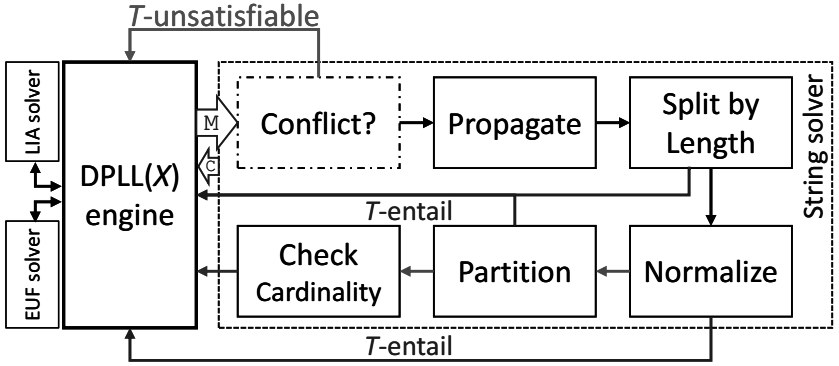
\includegraphics[width=0.7\linewidth]{pictures/proof_procedure.png}
   	\caption{Abstracted core proof procedure for string. The figure is sourced from \cite{main_phd}.}
   	\label{fig:proof_procedure}
   \end{figure}
  Figure \ref{fig:proof_procedure} shows the overall application strategy. The full list of derivation rules can be found in Figures from \ref{rules_1} to \ref{rules_5}. The four rules $\texttt{A-Prop},\texttt{S-Prop},\texttt{Len}$ and $\texttt{Len-Splite}$  in Figure \ref{rules_1} describe the interaction between arithmetic solver and string solver. This is achieved via the propagation of entailed constraints on the shared terms. This technique of cooperation between different theory solvers is well know as Nelson-Oppen method \cite{nelson_oppen}. The rule \texttt{S- Split}  tries to guess whether two strings are equal or not, while \texttt{L-Split} tries to guess whether two string variables have the same length.  Application of split rules causes the branching of the derivation tree. Whenever any new constraints are introduced to the set $S$, the procedure restart. Finally, when the procedure reached the saturated configuration, the rule \texttt{Card} makes sure that each bucket has been assigned big enough length. Detail about the individual rule can be found in \cite{main_phd} and in \cite{main-paper}.
 
 \begin{figure}
\scriptsize
\begin{minipage}{1.0\textwidth}
\begin{gather*}\label{eA1}
 \texttt{A-Prop} \frac{ S \models  \texttt{len} \ x \approx \texttt{len} \ y}{ A := A, \texttt{len} \ x \approx \texttt{len} \ y}\\
  \texttt{S-Prop} \frac{ A \models_{LIA}  \texttt{len} \ x \approx \texttt{len} \ y}{ S := S, \texttt{len} \ x \approx \texttt{len} \ y}\\
 \texttt{Len} \frac{ x \approx t \in \mathcal{C}(S) \ x \in \mathcal{V}(S)}{ A := A, \texttt{len} \ x \approx (\texttt{len} \ t) \downarrow}\\
 \texttt{Len-Split} \frac{ x \in \mathcal{V}(S \cup A) \ x: Str}{ S := S, x \approx \epsilon \parallel  A:= A, \texttt{len} \ x > 0}\\
 \texttt{A-Conflict} \frac{ A \models_{LIA} \perp }{ \texttt{unsat}}\\
 \texttt{R-Star} \frac{ s \ in \ star( set \ t) \in R \ s  \not\approx \epsilon \in \mathcal{C}(S)}{ S:= S, s \approx \textnormal{con}(t,z) \textnormal{R}:= \textnormal{R}, z \ in \ star \ (set \ t)}
\end{gather*}
\end{minipage}
\caption{ The rules for theory combination\cite{main-paper}. \texttt{R-Start} is handle cases with regular expression. }
\label{rules_1}
\end{figure}
 \begin{figure}
\begin{minipage}{1.0\textwidth}
\scriptsize
\begin{gather*}\label{eA1}
 \texttt{S-Cycle} \frac
 { t = \texttt{con}(t_1, \cdots, t_i, \cdots, t_n) \ t \in \mathcal{T}(S) \setminus C \ t_k \approx \epsilon \in \mathcal{C}(S) \ \textnormal{for all} \ k \in \{1,\cdots,n\} \setminus \{ i \} }
 { S := S, t \approx t_i \ C:=C (C, t) \setminus \{t_i\}   }\\
  \texttt{Reset} \frac{ }
  { \textnormal{F} := \phi, \textnormal{N} := \phi, \textnormal{B} := \phi}\\
   \texttt{S-Split} \frac
   { x, y \in \mathcal{V}(S) \ \ x \approx y, x \not\approx y \in \mathcal{C}(S) }
   { S := S, x \approx y \parallel S:= S, x \not\approx y}\\
      \texttt{S-Conflict} \frac
      { x \approx t \in \mathcal{C}(S) \ \ s \not\approx t \in \mathcal{C}(S)}
      { \textnormal{unsat}}\\
      \texttt{L-Split} \frac
       { x, y \in \mathcal{V}(S) \ \ x,y: \textnormal{Str}  \ \  S \not\models \texttt{len} \ x \not\approx \texttt{len} \ y}
       { S:= S, \texttt{len} \ x \approx \texttt{len} \ y \parallel S:=S, \texttt{len} \ x \not\approx \texttt{len} \ y}
\end{gather*}
\end{minipage}
\caption{Basic string derivation rules \cite{main-paper}.}
\label{rules_2}
\end{figure}

 \begin{figure}
\begin{minipage}{1.0\textwidth}
\scriptsize
\begin{gather*}\label{eA1}
 \bold{F-Form1} \frac
 { t = \textnormal{con}(t_1, \cdots,t_n) \ t \in \mathcal{T}(S) \setminus ( \mathcal{D}(F) \cup C)  \ \  N[t_1] = s_1 \cdots N[t_n] = s_n }
 { \textnormal{F} := \textnormal{F}, t \mapsto ( s_1, \cdots, s_n) \downarrow}\\
 \bold{F-Form2} \frac
 { l \in \mathcal{T}(S) \setminus \mathcal{D}(F)}
 { \textnormal{F} := \textnormal{F}, t \mapsto ( l)} \\
  \bold{N-Form1} \frac
  { [x] \not\in \mathcal{D}(N) \ \ s \in [x] \setminus ( C \cup \mathcal{V}(S)) \ \ F t= F s \textnormal{for all} \ t \in [x] \setminus ( C \cup \mathcal{V}(S)) }
  { \textnormal{N}:= \textnormal{N}, [x] \mapsto F s}\\
  \bold{N-Form2} \frac
  { [x] \not\in \mathcal{D}(N) \ \ [x] \subseteq  C \cup \mathcal{V}(S)} 
  { \textnormal{N}:= \textnormal{N}, [x] \mapsto (x)}
\end{gather*}
\null
\par\xdef\tpd{\the\prevdepth}
\end{minipage}
\caption{Normalization derivation rules. The letter \(l\) denotes a string constant.The rules are taken from \cite{main-paper} and they are in their original form.}
\label{rules_3}
\end{figure}
 \begin{figure}
\begin{minipage}{1.0\textwidth}
\scriptsize
\begin{gather*}\label{eA1}
 \texttt{F-Unify} \frac
 { F \ s = ( w,u,u_1) \ \ F \ t = (w, u,v_1)  s\approx t \in \mathcal{C}(S) \ S \models \texttt{len} \ u \approx \texttt{len} \ v }
 { S:= S, u \approx v}\\
  \texttt{F-Split} \frac
  {\parbox{3.2in}{$  F \ s = ( w,u,u_1) \ \ F \ t = (w, u,v_1)  s\approx t \in \mathcal{C}(S) \ S \models \texttt{len} u \approx \texttt{len} \ v  $ \\
       \hspace*{2.0cm}$ u \not\in \mathcal{V}(v_1) \ v \not\in \mathcal{V}(u_1)$}}
  { S:= S, u \approx con(v, z) \parallel  S:= S, v \approx con(u, z) }\\
  \texttt{F-Loop} \frac
  { F \ s = ( w,x,u_1) \ \ F \ t = (w, u,v_1, x, v_2)  \ s\approx t \in \mathcal{C}(S) \ x \not\in \mathcal{V}((v,v1))}
  { \parbox{3.6in}{$ S:= S, x \approx con(z_2, z),\ con(v,v1) \approx con(z_2,z_1),\ con(u_1) \approx con( z_1, z_2,v_2)$ \\
   \hspace*{2.0cm}$  R:=R, z \ in \ star(set \ con(z_1, z_2)) \ \ C:=C, t $}}
\end{gather*}
\end{minipage}
\caption{The rules for equality reduction \cite{main-paper}. The rule \texttt{F-Loop} is used to detect looping problem.}
\label{rules_4}
\end{figure}
 \begin{figure}
\begin{minipage}{1.0\textwidth}
\scriptsize
\begin{gather*}\label{eA1}
 \texttt{D-Base} \frac
 { s \in \mathcal{T}(S) \ \ s: \textnormal{Str}  \ \  S \models \textnormal{len} \ s \approx \textnormal{len}_B \textnormal{ for no }  B \in B }
 { B:= B, \{ [s]\}}\\
  \texttt{Card} \frac
  {B \in B \ \ |B| > 1}
  { A:= A, \textnormal{len}_B >  \lfloor  log_{| \mathcal{A}|}  \ ( |B| -1) \rfloor }\\
  \texttt{D-Add} \frac
  { \parbox{3.3in}{\hspace*{0.5cm} $s \in \mathcal{T}(S) \ \ s: \textnormal{Str} \ \ B = \textnormal{B'}, B \   S \models \textnormal{len} \ s \approx \textnormal{len}_B  [s]  \not\in B 
  		$ \\
  		\hspace*{0.8cm}$  		\textnormal{ for all }  e \in B \textnormal{ there are } w, u,u_1, v,v_1 \textnormal{ such that} 
  		 $ \\
  		 \hspace*{0.0cm}$ (N [s] = (w, u,u_1), N e = (w, v,v1), \ S \models \textnormal{len} \ u \approx \textnormal{len} v, u \not\approx v \in \mathcal{C}(S))$}}
  { B:= B', ( B \cup \{ [s]\})}\\
  \texttt{D-Split} \frac
  { \parbox{4.0in}{\hspace*{1.5cm} $s \in \mathcal{T}(S) \ \ s: \textnormal{Str} \ \ B = \textnormal{B'}, B \   S \models \textnormal{len} \ s \approx \textnormal{len}_B  [s]  \not\in B \ e \in B   		 
  		$ \\
  		\hspace*{2cm}$ (N [s] = (w, u,u_1), N e = (w, v,v1), \ S \models \textnormal{len} \ u \not\approx \textnormal{len}\ v $}}
  {  S:=S, u \approx con(z_1, z_2), len \ z_1 \approx len \ v  \parallel  S:=S, v \approx con(z_1, z_2), len \ z_1 \approx len \ u}
  \end{gather*}
 \end{minipage}
\caption{The rules for dis-equality reduction\cite{main-paper}.}
\label{rules_5}
\end{figure}
    
    
%\begin{figure}
	\centering
	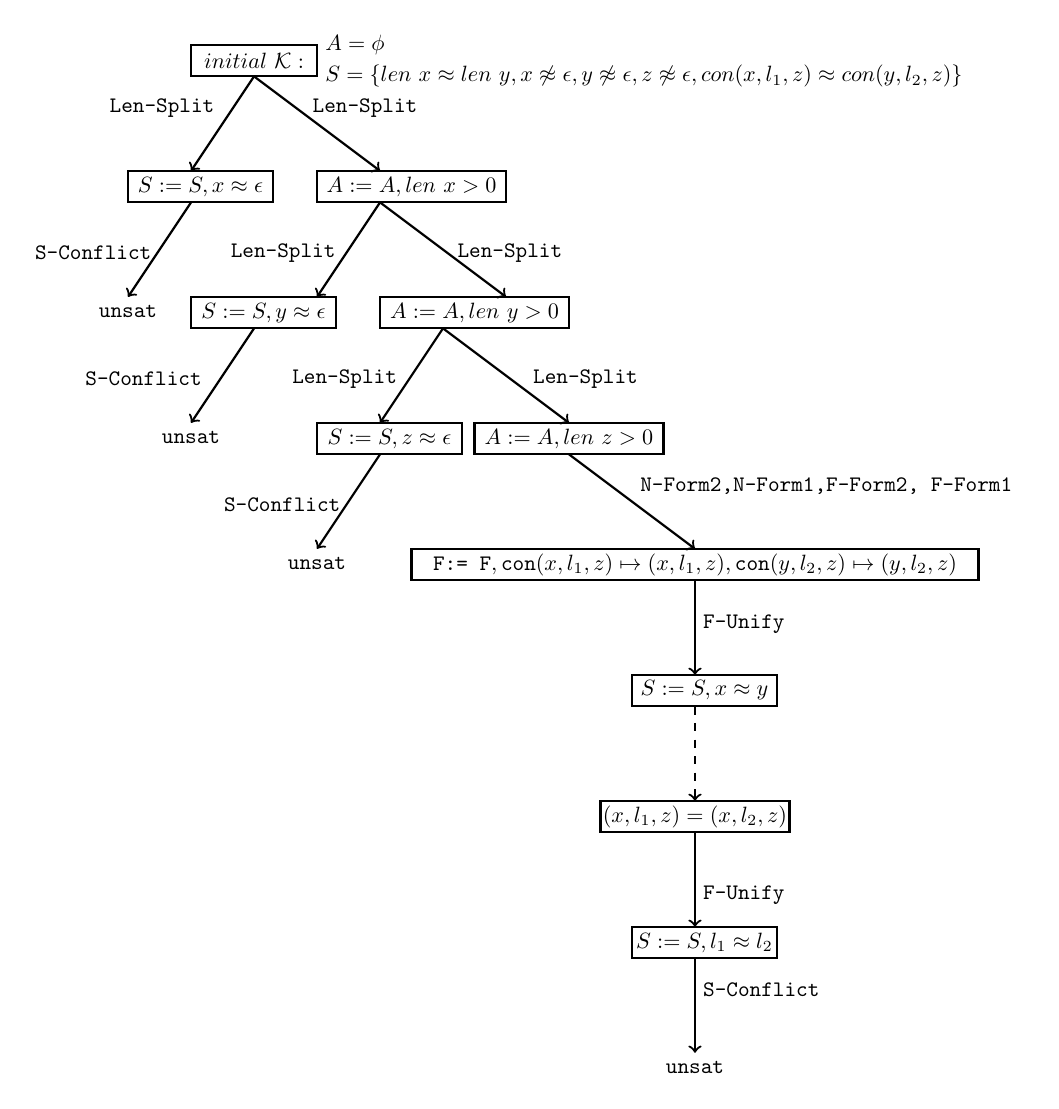
\begin{tikzpicture}[thick,scale=0.8, every node/.style={transform shape}]
	
	\node [right] at (3,20) { $ A=\phi $};
	\node [right] at (3,19.5) { $ S=\{  len \ x \approx len \ y, x \not\approx \epsilon, y \not\approx \epsilon,
		z \not\approx \epsilon, con (x, l_1,z) \approx con (y, l_2, z)\} $}; 
	 
    \draw (1,20) rectangle (3,19.5) node[pos=.5] {$ initial \ \mathcal{K}:$};
	
	\draw [->] (2,19.5) -- (1,18);
	\node [left] at (1.5,19) {$\texttt{Len-Split}$};
	
	\draw [->] (2,19.5) -- (4,18);
	\node [right] at (2.8,19) {$\texttt{Len-Split}$};
	
	
	\draw (0,18) rectangle (2.3,17.5) node[pos=.5] {$S:=S, x\approx \epsilon$};
	\node [rectangle, below] at (1,18) {};
	
	
	\draw (3,18) rectangle (6,17.5) node[pos=.5] {$A:=A, len \ x  > 0$};
	\node [rectangle, below] at (4,18) {};
	
	\draw [->] (1,17.5) -- (0,16);
	\node [left] at (0.5,16.7) {$\texttt{S-Conflict}$};
	
	\draw [->] (4,17.5) -- (3,16);
	\node [right] at (1.5,16.7) {$\texttt{Len-Split}$};
	\draw [->] (4,17.5) -- (6,16);
	\node [right] at (5.1,16.7) {$\texttt{Len-Split}$};
	
	\node [below] at (0,16) {$\texttt{unsat}$};
	\draw (1,16) rectangle (3.3,15.5) node[pos=.5] {$S:=S, y\approx \epsilon$};
	\node [below] at (2,16) {};
	\draw (4,16) rectangle (7,15.5) node[pos=.5] {$A:=A, len \ y  > 0$};
	\node [below] at (5,16) {};
	
	\draw [->] (2,15.5) -- (1,14);
	\node [left] at (1.3,14.7) {$\texttt{S-Conflict}$};
	\draw [->] (5,15.5) -- (4,14);
	\node [left] at (4.4,14.7) {$\texttt{Len-Split}$};	
	\draw [->] (5,15.5) -- (7,14);
	\node [right] at (6.3,14.7) {$\texttt{Len-Split}$};
	
	
	\node [below] at (1,14) {$\texttt{unsat}$};
	\draw (3,14) rectangle (5.3,13.5) node[pos=.5] {$S:=S, z\approx \epsilon$};
	\node [below] at (4,14) {};
	\draw (5.5,14) rectangle (8.5,13.5) node[pos=.5] {$A:=A, len \ z  > 0$};
	\node [below] at (7,14) {};


	\draw [->] (4,13.5) -- (3,12);
	\node [left] at (3.5,12.7) {$\texttt{S-Conflict}$};
	\draw [->] (7,13.5) -- (9,12);
    \node [right] at (8,13) {$\texttt{N-Form2,N-Form1,F-Form2, F-Form1 }$};
    

	
	\node [below] at (3,12) {$\texttt{unsat}$};
	\draw (4.5,12) rectangle (13.5,11.5) node[pos=.5] {$\texttt{F:= F},\texttt{con}(x,l_1,z)\mapsto (x,l_1,z),\texttt{con}(y,l_2,z)\mapsto(y,l_2,z)$};
	\node [below] at (9,12) {};
	
	\draw [->] (9,11.5) -- (9,10);
	\node [right] at (9,10.8) {$\texttt{F-Unify}$};
	
	\draw (8,10) rectangle (10.3,9.5) node[pos=.5] {$S:=S, x\approx y$};
	\node [below] at (9,10) {};
	
	\draw [dashed,->] (9,9.5) -- (9,8);
	
	\draw (7.5,8) rectangle (10.5,7.5) node[pos=.5] {$( x, l_1, z ) = (x, l_2,z)$};
	\node [below] at (9,8) {};
	
	\draw [->] (9,7.5) -- (9,6);
	\node [right] at (9,6.5) {$\texttt{F-Unify}$};
	
	\draw (8,6) rectangle (10.3,5.5) node[pos=.5] {$S:=S, l_1 \approx l_2$};
	\node [below] at (9,6) {};
	
	\draw [->] (9,5.5) -- (9,4);
	\node [right] at (9,5) {$\texttt{S-Conflict}$};
	
	\node [below] at (9,4) {$\texttt{unsat}$};
	
	
	
	
	
	
	\end{tikzpicture}
	\caption{The derivation tree for example 1. Here $l_1, l_2 $ are distinct constants of same length.}
\end{figure}	





\begin{figure}[ht]
	\centering
 	\begin{minipage}[t]{0.45\linewidth}
 		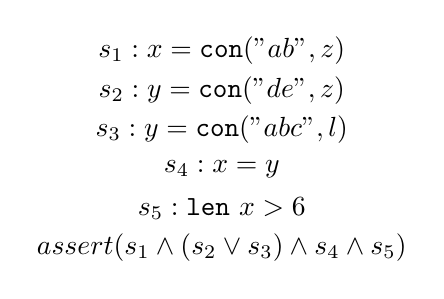
\begin{tikzpicture}[->,>=stealth',
 		shorten >=1pt,auto,node distance=0.5cm,thick,
 		main node/.style={rectangle,draw}, text node/.style={rectangle}]
 		
 		
 		\node  (s1){$s_1: x =  \texttt{con}("ab", z) $};
 		\node  (s2) [below of=s1] {$s_2: y =  \texttt{con}("de", z) $};
 		\node  (s3) [below of=s2] {$s_3: y =  \texttt{con}("abc", l)$};
 		\node  (s4) [below of=s3] {$s_4: x =  y$};
 		\node  (s5) [below of=s4] { $s_5: \texttt{len}\  x > 6$};
 		\node  (s6) [below of=s5] {$assert( s_1 \wedge (s_2 \vee s_3 ) \wedge s_4 \wedge s_5)$};
 		
 		
 		\end{tikzpicture}
 	\end{minipage}
	\quad
	\centering
	\begin{minipage}[t]{0.45\linewidth}
		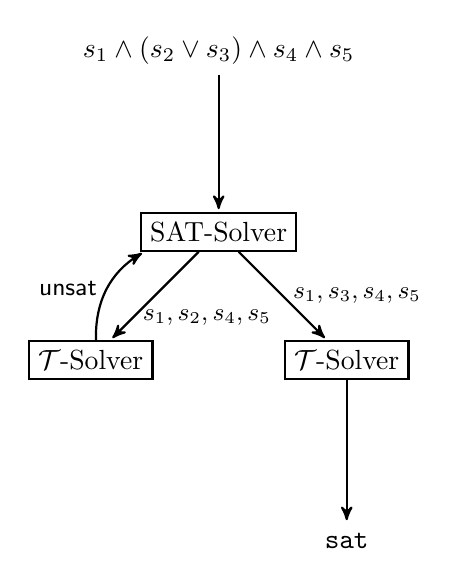
\begin{tikzpicture}[->,>=stealth',
		shorten >=1pt,auto,node distance=2.3cm,thick,
		main node/.style={rectangle,draw}, text node/.style={rectangle}]
		
		\node (root) {$ s_1 \wedge (s_2 \vee s_3 ) \wedge s_4 \wedge s_5$};
		\node[main node] (sat-solver) [below of=root] {SAT-Solver};
		\node[main node] (t-solver-1) [below left of=sat-solver] {$\mathcal{T}$-Solver};
		\node[main node] (t-solver-2) [below right of=sat-solver] {$\mathcal{T}$-Solver};	
		\node[text node] (sat) [below of=t-solver-2] {$ \texttt{sat}$};
		
		
		\path[every node/.style={font=\sffamily\small}]
		(root) edge node [left] {} (sat-solver)	
		
		(sat-solver) edge node [right, near end] { $s_1 ,s_2 ,  s_4, s_5$} (t-solver-1)
		(sat-solver) edge node [right] {$s_1 ,s_3 ,  s_4, s_5$} (t-solver-2)	
		(t-solver-1) edge [bend left] node [left] {unsat} (sat-solver)	
		(t-solver-2) edge  node [right] {} (sat);
		\end{tikzpicture}
	\end{minipage}
	\caption{On the left the set of constraints and the boolean formula. And on the right side the interaction with SAT-Solver core and theory solver is shown.}
	\label{smt_example_1_2}
\end{figure}

	\begin{figure}
		\centering	
		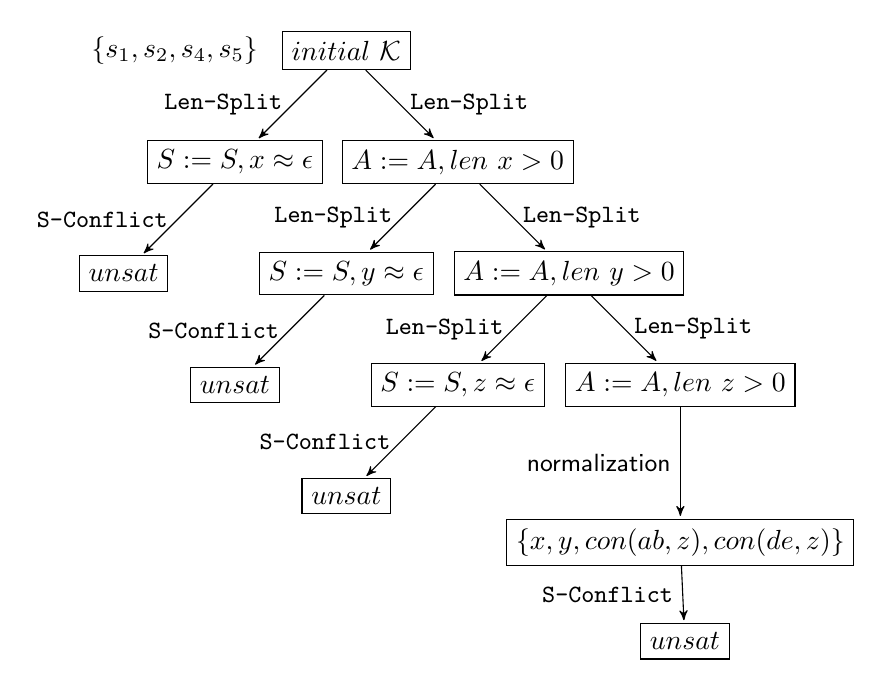
\begin{tikzpicture}[->,>=stealth',
		shorten >=1pt,auto,node distance=2cm,thin,
		main node/.style={rectangle,draw}, text node/.style={rectangle}]
		
		
		\node [left] at (-10mm,0) {$ \{s_1, s_2, s_4,  s_5\}$};
		\node[main node] (a) {$initial\ \mathcal{K}$};
		\node[main node] (b) [below left of=a] {$S:=S, x\approx \epsilon$};
		\node[main node] (c) [below right of=a] {$A:=A, len\ x > 0$};
		
		\node[main node] (d) [below left of=b] {$unsat$};
		\node[main node] (e) [below left of=c] {$S:=S, y\approx \epsilon$};
		\node[main node] (f) [below right of=c] {$A:=A, len\ y > 0$};
		
		\node[main node] (g) [below left of=e] {$unsat$};
		\node[main node] (h) [below left of=f] {$S:=S, z\approx \epsilon$};
		\node[main node] (i) [below right of=f] {$A:=A, len\ z > 0$};
		
		\node[main node] (j) [below left of=h] {$unsat$};
		\node[main node] (k) [below of=i] {$\{ x,y,con(ab,z),con(de,z)\}$};
		
		\node [draw] (l) at (43mm,-75mm)  {$unsat$};
		
		
		\path[every node/.style={font=\sffamily\small}]
		(a) edge node [left] {\texttt{Len-Split}} (b)
		(a) edge node [right] {\texttt{Len-Split}} (c)
		(b) edge node [left] {\texttt{S-Conflict}} (d)
		(c) edge node [left] {\texttt{Len-Split}} (e)
		(e) edge node [left] {\texttt{S-Conflict}} (g)
		(c) edge node [right] {\texttt{Len-Split}} (f)
		(f) edge node [left] {\texttt{Len-Split}} (h)
		(f) edge node [right] {\texttt{Len-Split}} (i)
		(h) edge node [left] {\texttt{S-Conflict}} (j)
		(i) edge node [left] {normalization} (k)
		(k) edge node [left] {\texttt{S-Conflict}} (l);
		
		\end{tikzpicture}			
		\caption{The branch of derivation tree, which ends up in \texttt{unsat}.}
		\label{leftDerivationTree}
	\end{figure}
	\begin{figure} 	
		\centering
		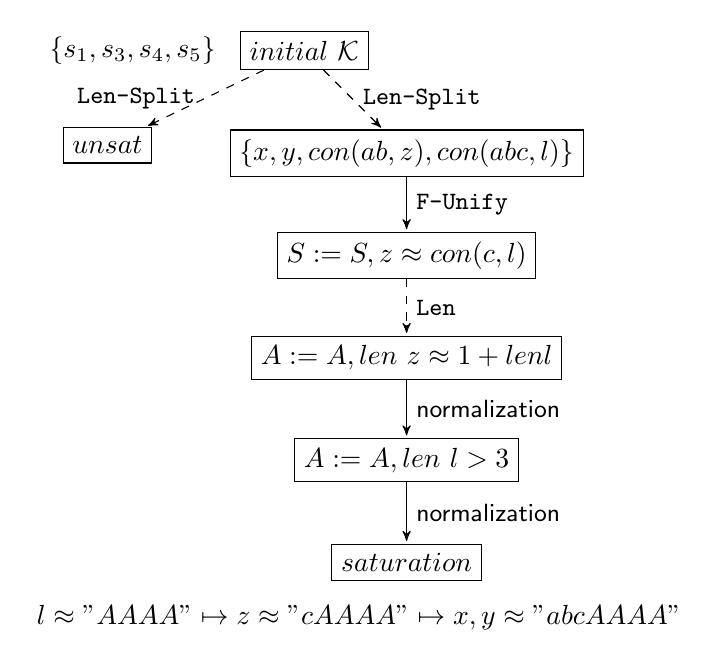
\begin{tikzpicture}[->,>=stealth',
		shorten >=1pt,auto,node distance=1.3cm,thin,
		main node/.style={rectangle,draw}, text node/.style={rectangle}]
		
		
		\node [left] at (-10mm,0) {$ \{s_1, s_3, s_4,  s_5\}$};
		\node[main node] (a) {$initial\ \mathcal{K}$};
		\node (dummy) [below of=a] {};
		%\node[main node] (b) [left of=dummy] {$unsat$};		
		\node [draw] (b) at (-25mm,-12mm)  {$unsat$};
		\node[main node] (c) [right of=dummy] {$\{ x,y,con(ab,z),con(abc,l)\}$};
		\node[main node] (d) [below of=c] {$S:=S, z \approx con(c, l)$};
		\node[main node] (e) [below of=d] {$A:=A, len\ z \approx 1 + len l$}; 
		\node[main node] (f) [below of=e] {$A:=A, len\ l > 3$};
		\node[main node] (g) [below of=f] {$saturation$};
		
		\node at (7mm,-72mm) {$ l \approx "AAAA" \mapsto z \approx "cAAAA" \mapsto x, y\approx "abcAAAA"$};
		
		\path[every node/.style={font=\sffamily\small}]
		(a) edge [dashed] node [left] {\texttt{Len-Split}} (b)
		(a) edge [dashed] node [right] {\texttt{Len-Split}} (c)
		(c) edge  node [right] {\texttt{F-Unify}} (d)
		(d) edge [dashed] node [right] {\texttt{Len}} (e)
		(e) edge  node [right] {normalization} (f)
		(f) edge  node [right] {normalization} (g);
		
		
		\end{tikzpicture}			
		\caption{The branch of derivation tree, which ends up in saturation.}
		\label{rightDerivationTree}
	\end{figure}		
	
	

    \section{Example}
In this section, we will use the example formula \ref{mainConstraint} to explain how the decision procedure works. Consider the five constraints $s_1,s_2, s_3,s_4,s_5$ on the left side of Figure \ref{smt_example_1_2}. Since the SAT core cannot interpret the constraints, it treats them as five independent boolean variables and tries to assign values to them. The core starts by setting $s_1, s_4$ and $s_5$ to \texttt{true}. Then the SAT core choose true for $s_2$ before $s_3$.  Now the selected constraints $\{ s_1,s_2, s_4,s_5\}$  are forwarded to the theory solver. This is shown as the left branch of the tree on the right side of Figure \ref{smt_example_1_2}. The theory solver will answer \texttt{unsat} for this set of constraints. The SAT core backtracks and tries the other option. That is the SAT core choose $s_3$ and ask theory solver to solve the new set of constraints  $\{ s_1,s_3, s_4,s_5\}$. This is shown as the right branch of the tree on the right of Figure \ref{smt_example_1_2}. The theory solver eventually finds a satisfying solution in this branch. 

\begin{description}
	\item[Left derivation tree:] The input constraints are: $A = \{ \texttt{len}\ x > 6\}$ and $S= \{ x = \texttt{con}('ab', z), y = \texttt{con}('de', z), x = y\}$.
		
	The procedure starts with by applying \texttt{Reset}. Then it tries to find conflict by applying \texttt{S-Conflict} and \texttt{A-Conflict} and fails to find any contradiction in the current constraints. 
	
	The procedure tries to apply \texttt{A-Prop} and \texttt{S-Prop}. The constraints in different theories fail to induce new constraint for other. 
	
	Now the procedure keeps trying to apply rules \texttt{Len} and \texttt{Len-Split}. The application of these split rule causes the tree to branch into new configurations. However, all the branches are closed with respect to the rule \texttt{S-Conflict}. This is shown in the left branches in Figure \ref{leftDerivationTree}.
	
	Now for the non closing configuration, the procedure goes on to compute the normal forms. $x = y$ causes  $\texttt{con} ('ab', z) ,\texttt{con} ('de', z)$ to be classified as equivalent term. Further application of rule  \texttt{F-Unify} causes to introduce $'ab' = 'de'$ into $S$ and eventually this branch get closed by \texttt{S-Conflict}. Thus the procedure decides that, the given set of constraints are unsatisfiable.
	
	
	\item[Right derivation tree:] The input constraints are: $A = \{ \texttt{len}\ x > 6\}$ and $S= \{ x = \texttt{con}('ab', z), y = \texttt{con}('abc', l), x = y\}$. The derivation tree is shown in Figure \ref{rightDerivationTree}.
		
	Similar to the left derivation tree, the procedure reaches a configuration, where the string equivalence classes are like  $\{ x,y, \texttt{con}('ab', z), \texttt{con}('abc', l)\}, \{ z\}, \{ l\}$. Application of the rule \texttt{F-Unify} causes the introduction of new constraints $ z = \texttt{con}('c', l)$. The procedure restarts with new equivalence classes  $\{ x,y, \texttt{con}('ab', z), \texttt{con}('abc', l)\}, \{ z,  \texttt{con}('c', l)\}, \{ l\}$ with the application of \texttt{Reset}. The new constraint in $S$ induces new constraints in $A$. That application of \texttt{Len} causes $A: =A , \texttt{len} \ z = 1 + \texttt{len} \ l$. At this point the procedure starts to compute the normal forms by applying different rules. Eventually the constraint $\texttt{len}\ l > 3$ is computed and a saturated configuration is reached. As no more rule application is not possible at this configuration. Thus the procedure concludes that the problem is satisfiable. 
	
	Finally, for each buckets an arithmetic constraint on the minimum length is added. For example, $\texttt{len}\ l > 3$ causes the length of the bucket which contain $l$ to be 4. Now it is trivial to find a satisfying assignment. that if $ l = 'AAAA'$ then $ z = 'cAAAA'$ and $x, y = 'abcAAAA'$.
	
\end{description}
    
    %\subsection{Examples}
Now we try to illustrate the procedure's workings with respect of two example. First example shows how the procedure conclude $unsat$ for a set of constraints which are unsatisfiable. And the second shows how the procedure finds a saturated configuration for a set of constraints which are satisfiable. Both the examples are taken from \cite{main-paper}.
\begin{description}			
	\item[Example 1:] The input constraints are: $ A = \phi$ and $S = \{ \texttt{len}(x) \approx
	\texttt{len}(y), x \not\approx \epsilon, y\not\approx \epsilon, z \not\approx \epsilon, \texttt{con}(x, l_1, z) \approx \texttt{con}(y, l_2, z)\}$, where $l_1$, $l_2$ are distinct constants of the same length.	

The procedure starts with $step\ 0$ by applying \texttt{Reset}. It tries to find conflicts by applying   \texttt{S-Conflict} and \texttt{A-Conflict}. Since the arithmetic constraint set $A$ is empty and there are no contradicting string constraints in $S$, $check\ for\ contradiction$ fails. 

The procedure tries the step $propagate$. For this example this step does not introduce any new constraint in $S$, as $A$ is empty. Now the procedure applies \texttt{Len} and \texttt{Len-Split} repeatedly as long as there is possible application. The application of these two splitting rules causes the branching of the derivation tree. However, all branches are closed by rule  \texttt{S-Conflict} expect one. This is shows in Figure as the left branches of each configuration. 

In this non closing configuration, the string equivalence classes are $\{x\}, \{y\}, \{z\}, \{l_1\}, \{l_2\}, \{\epsilon\},$ and $\{ \texttt{con}(x, l_1, z), \texttt{con}(y, l_2, z)\}$. Now the procedure goes on to compute normal forms by applying \texttt{N-Form2}, \texttt{F-Form2} and \texttt{N-Form1}.The flat forms  \texttt{F} $\texttt{con}(x, l_1, z) = (x, l_1, z)$ and \texttt{F} $\texttt{con}(y, l_2, z) = (y, l_2, z)$ are computed by \texttt{F-Form1}. Then \texttt{F-Unify} is applied to add the equality $x \approx y$ to $S$. This causes the procedure to restart, but with an extended constraints set. Which induces a new equivalence classes $ \{x, y\}, \{z\}, \{l_1\}, \{l_2\}, \{\epsilon\}$, and $\{\texttt{con}(x, l_1, z), \texttt{con}(y, l_2, z)\}$. After similar steps, the procedure reached a stage where it computes the flat forms $(x, l_1, z)$ and $(x, l_2, z)$ for the  corresponding equivalence class,
by choosing $x$ as representative of $y$. At this point the procedure applies rule \texttt{F-Unify} again. This introduces a new equality $l_1 \approx l_2$ to $S$ and eventually derives \texttt{unsat} with \texttt{S-Conflict}. That is the procedure ended up with a derivation tree where each branch is closed and conclude that the input constraints are unsatisfiable.  The resulting derivation tree is shown in figure .

\begin{figure}
	\centering
	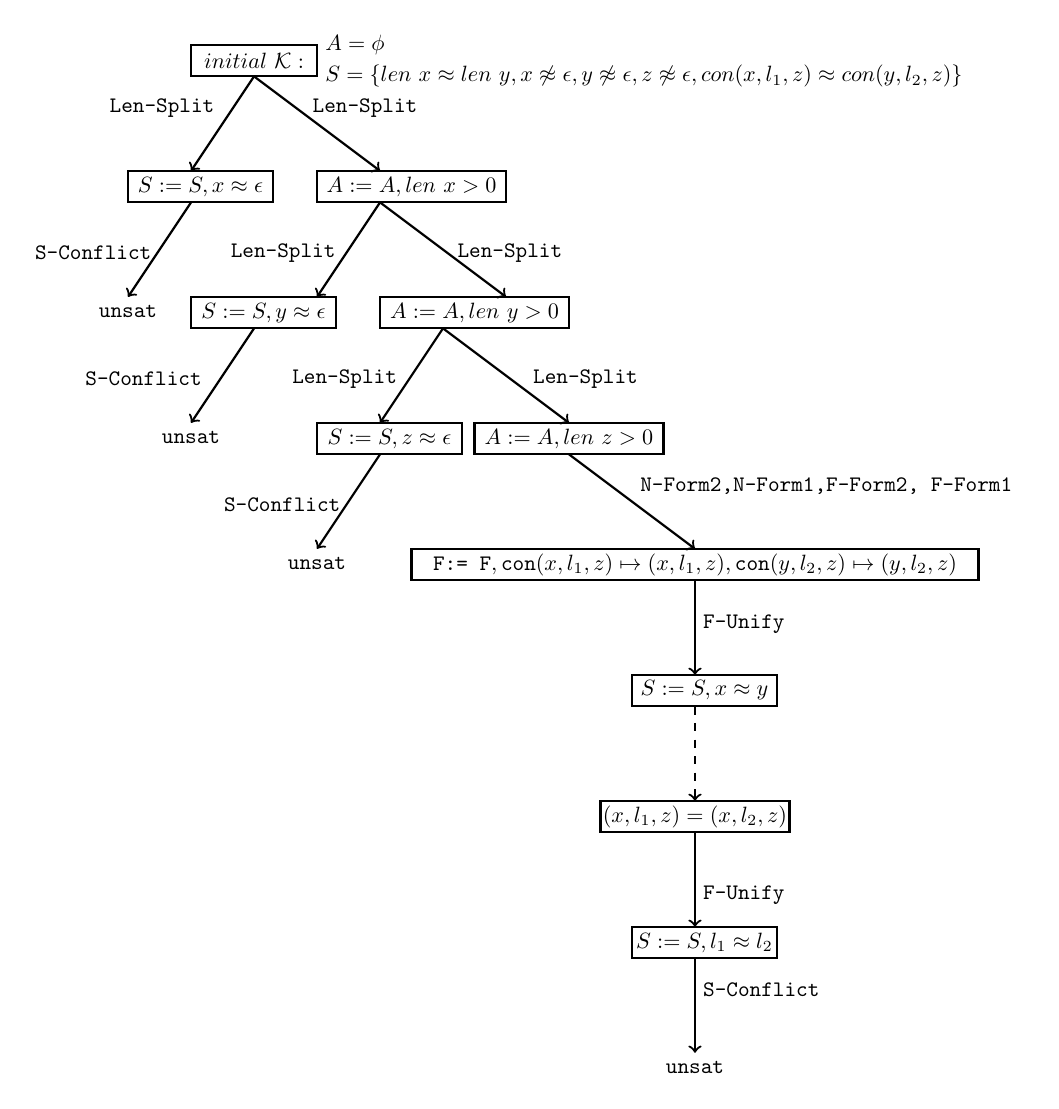
\begin{tikzpicture}[thick,scale=0.8, every node/.style={transform shape}]
	
	\node [right] at (3,20) { $ A=\phi $};
	\node [right] at (3,19.5) { $ S=\{  len \ x \approx len \ y, x \not\approx \epsilon, y \not\approx \epsilon,
		z \not\approx \epsilon, con (x, l_1,z) \approx con (y, l_2, z)\} $}; 
	 
    \draw (1,20) rectangle (3,19.5) node[pos=.5] {$ initial \ \mathcal{K}:$};
	
	\draw [->] (2,19.5) -- (1,18);
	\node [left] at (1.5,19) {$\texttt{Len-Split}$};
	
	\draw [->] (2,19.5) -- (4,18);
	\node [right] at (2.8,19) {$\texttt{Len-Split}$};
	
	
	\draw (0,18) rectangle (2.3,17.5) node[pos=.5] {$S:=S, x\approx \epsilon$};
	\node [rectangle, below] at (1,18) {};
	
	
	\draw (3,18) rectangle (6,17.5) node[pos=.5] {$A:=A, len \ x  > 0$};
	\node [rectangle, below] at (4,18) {};
	
	\draw [->] (1,17.5) -- (0,16);
	\node [left] at (0.5,16.7) {$\texttt{S-Conflict}$};
	
	\draw [->] (4,17.5) -- (3,16);
	\node [right] at (1.5,16.7) {$\texttt{Len-Split}$};
	\draw [->] (4,17.5) -- (6,16);
	\node [right] at (5.1,16.7) {$\texttt{Len-Split}$};
	
	\node [below] at (0,16) {$\texttt{unsat}$};
	\draw (1,16) rectangle (3.3,15.5) node[pos=.5] {$S:=S, y\approx \epsilon$};
	\node [below] at (2,16) {};
	\draw (4,16) rectangle (7,15.5) node[pos=.5] {$A:=A, len \ y  > 0$};
	\node [below] at (5,16) {};
	
	\draw [->] (2,15.5) -- (1,14);
	\node [left] at (1.3,14.7) {$\texttt{S-Conflict}$};
	\draw [->] (5,15.5) -- (4,14);
	\node [left] at (4.4,14.7) {$\texttt{Len-Split}$};	
	\draw [->] (5,15.5) -- (7,14);
	\node [right] at (6.3,14.7) {$\texttt{Len-Split}$};
	
	
	\node [below] at (1,14) {$\texttt{unsat}$};
	\draw (3,14) rectangle (5.3,13.5) node[pos=.5] {$S:=S, z\approx \epsilon$};
	\node [below] at (4,14) {};
	\draw (5.5,14) rectangle (8.5,13.5) node[pos=.5] {$A:=A, len \ z  > 0$};
	\node [below] at (7,14) {};


	\draw [->] (4,13.5) -- (3,12);
	\node [left] at (3.5,12.7) {$\texttt{S-Conflict}$};
	\draw [->] (7,13.5) -- (9,12);
    \node [right] at (8,13) {$\texttt{N-Form2,N-Form1,F-Form2, F-Form1 }$};
    

	
	\node [below] at (3,12) {$\texttt{unsat}$};
	\draw (4.5,12) rectangle (13.5,11.5) node[pos=.5] {$\texttt{F:= F},\texttt{con}(x,l_1,z)\mapsto (x,l_1,z),\texttt{con}(y,l_2,z)\mapsto(y,l_2,z)$};
	\node [below] at (9,12) {};
	
	\draw [->] (9,11.5) -- (9,10);
	\node [right] at (9,10.8) {$\texttt{F-Unify}$};
	
	\draw (8,10) rectangle (10.3,9.5) node[pos=.5] {$S:=S, x\approx y$};
	\node [below] at (9,10) {};
	
	\draw [dashed,->] (9,9.5) -- (9,8);
	
	\draw (7.5,8) rectangle (10.5,7.5) node[pos=.5] {$( x, l_1, z ) = (x, l_2,z)$};
	\node [below] at (9,8) {};
	
	\draw [->] (9,7.5) -- (9,6);
	\node [right] at (9,6.5) {$\texttt{F-Unify}$};
	
	\draw (8,6) rectangle (10.3,5.5) node[pos=.5] {$S:=S, l_1 \approx l_2$};
	\node [below] at (9,6) {};
	
	\draw [->] (9,5.5) -- (9,4);
	\node [right] at (9,5) {$\texttt{S-Conflict}$};
	
	\node [below] at (9,4) {$\texttt{unsat}$};
	
	
	
	
	
	
	\end{tikzpicture}
	\caption{The derivation tree for example 1. Here $l_1, l_2 $ are distinct constants of same length.}
\end{figure}	


	
	
\end{description}
\begin{description}			
	\item[Example 2:] The input constraints are: $ A = \phi$ and $S = \{ \texttt{len}(x) \approx
	\texttt{len}(y), x \not\approx \epsilon, z \not\approx \epsilon, \texttt{con}(x, l_1, z) \not\approx \texttt{con}(y, l_2, z)\}$, with $l_1$, $l_2$ are distinct constants of the same length.
	
	
	Similar to the previous example, the procedure reaches a configuration where the string equivalence classes are $ \{x\}, \{y\}, \{z\}, \{l_1\}, \{l_2\}, \{\epsilon\},\{ \texttt{con}(x, l_1, z)\}$ and,$\{\texttt{con}(y, l_2, z)\}$.
	In this case, the procedure attempts to partition the the equivalence classes into buckets. It fails to create the full partition, as rule \texttt{D-Base}  nor rule \texttt{D-Add} is applicable to $[y]$ because of $S \models \texttt{len} \ x \approx \texttt{len} \ y$ and  $x \not\approx y \not\in \mathcal{C}(S)$.  
	
	In such a case the procedure tries to guess by applying rule \texttt{S-Split} to $x$ and $y$. It case two branches in the derivation tree, one for $x \approx y$ and another for $x \not\approx y$.  
		
	After similar steps as in previous example, the procedure can derive a configuration where the string equivalence classes are $ \{x\}, \{y\}, \{z\}, \{l_1\}, \{l_2\}, \{\epsilon\},\{ \texttt{con}(x, l_1, z)\}$ and,$\{\texttt{con}(y, l_2, z)\}$. After computing normal forms for these classes, it attempts to	construct a partition \texttt{B} of them into buckets. However, notice that if it adds {[x]},say, to \texttt{B} using \texttt{D-Base}, then neither \texttt{D-Base} (since $S \models \texttt{len} \ x \approx \texttt{len} \ y$) nor \texttt{D-Add} (since $x \not\approx y \not\in \mathcal{C}(S)$ ) is applicable to $[y]$. So it applies \texttt{S-Split} to $x$ and $y$. In the branch where $ x \approx y$, the procedure subsequently restarts as new constraints are introduced to $S$. Eventually the procedure computes normal forms and succeeds in making a full partition of \texttt{B}. The procedure places $[\texttt{con}(x, l_1, z)]$ and $[\texttt{con}(y, l_2, z)]$ into the same bucket using \texttt{D-Add}, which applies because their corresponding normal forms are $(x, l_1, z)$ and $(x, l_2, z)$ respectively. Any further rule applications lead to branches with  a saturated configuration. Thus the procedure concludes that the problem is satisfiable. For each of the branches with saturated configuration satisfying models can be generated.
\end{description}
Here in this section we have tried to explore the inner working of the decision procedure. According to the authors \cite{main-paper}, the presented version the procedure is a simplified one. The procedure and derivation rules, which are implemented as part of cvc4 is much more complex and elaborate.
    %\subsection{Integration  into SMT solver architecture}
\label{sec:Implementation in DPLLt}
In this section we will explain, how the string theory solver is integrated into modern DPLL($T$) framework.
We will briefly discuss the issues of $theory\ propagation$, $lemma\ learning$ and $conflict\ analysis$.

 
Modern SMT solvers combine a SAT solver with multiple specialized $theory\ solvers$. The SAT solver maintain an evolving set $F$ of clauses and a set $M$ of literals representing partial assignment. The whole process is derived by the SAT solver. It periodically consults the theory solver, to find whether $M$ is satisfiable in its theory. The literals of an assignment $M$ are partitioned into string constraints, arithmetic constraints. These sets are subsequently given to the independent solvers. The rules \texttt{A-Prop} and \texttt{S-Prop} model the mechanism for $theory\ combination$. This mechanism is known as Nelson-Oppen theory combination \cite{nelson_oppen}, where the entailed equalities are communicated between multiple solvers. The rule \texttt{A-Conflict} modeled the satisfiability checking done by the arithmetic solver. As there is no additional requirement for the arithmetic solver, a standard theory solver for linear integer arithmetic can be used. 

The case splitting done by the string solver (with rules \texttt{S-Split} and \texttt{L-Split}) is achieved by means of the $splitting\ on\ demand$ paradigm, in which a solver may add theory lemmas to $F$ consisting of clauses possibly with literals not occurring in $M$.  This approach of $lemma\ learning$ is very efficient as new lemmas are introduced only when it is needed.  Similarly, the rules \texttt{Len}, \texttt{Len-Split}, and \texttt{Card} are involved in introduction of new constraints into \texttt{A}. This is done by the string solver by adding lemmas to ${F}$ containing arithmetic constraints. For example, if $x \approx \texttt{con}(y, z) \in \mathcal{C}(\texttt{S})$, the solver may add a lemma of the form $ \psi \Rightarrow \texttt{len}\ x \approx \texttt{len}\ y + \texttt{len}\ z$ to $F$, where $\psi$ is a conjunction of literals from $M$ entailing $x \approx \texttt{con}(y, z)$, after which the conclusion of this lemma is added to $M$.

When a theory solver determines that $M$ is unsatisfiable, it produces a $conflict\ clause$ to support the decision. A $conflict\ clause$ is the negation of an unsatisfiable subset of $M$. Whenever the string solver introduces any equality to \texttt{S}, it also maintains an explanation $ \psi_{s,t}$ for each equality $s \approx t$. An explanation $\psi_{s,t}$ is a conjunction of string constraints in $M$ such that $\psi_{s,t} \models s \approx t$. When a configuration is decided to be unsatisfiable by rule \texttt{S-Conflict},that is, when $ s \approx t, s \not\approx t \in \mathcal{C}(\texttt{S})$ for some $s, t,$ it replaces the occurrence of $s \approx t$ with its corresponding explanation $\psi$, and then replaces the equalities in $\psi$ with their corresponding explanation, and so on, until $\psi$ contains only equalities from $M$. Finally, it reports the conflict clause 
$ \psi \Rightarrow s \approx t$.

The core idea of the above explanations are taken from \cite{main-paper}.
    \section{Correctness}
\label{sec:Correctness}
The procedure is $refutation\ sound$, that is when the procedure answers \texttt{unsat}, it can be trusted even for strings of unbounded length. And the procedure is $solution\ sound$, that is when the procedure answers $sat$, it can be trusted. In the original paper \cite{main-paper}, the authors have claimed that they have a version of the procedure which is also $solution\ complete$, that is when the procedure answers $sat$, it will eventually get a model by finite model finding. However, the procedure  is $refutation\ complete$, that is for an unsatisfiable set of constraints the procedure may not terminate. More detail on the correctness properties and the proofs of these theorem can be found in \cite{main_phd}.
    
    
    
    %\begin{figure}
	\centering
	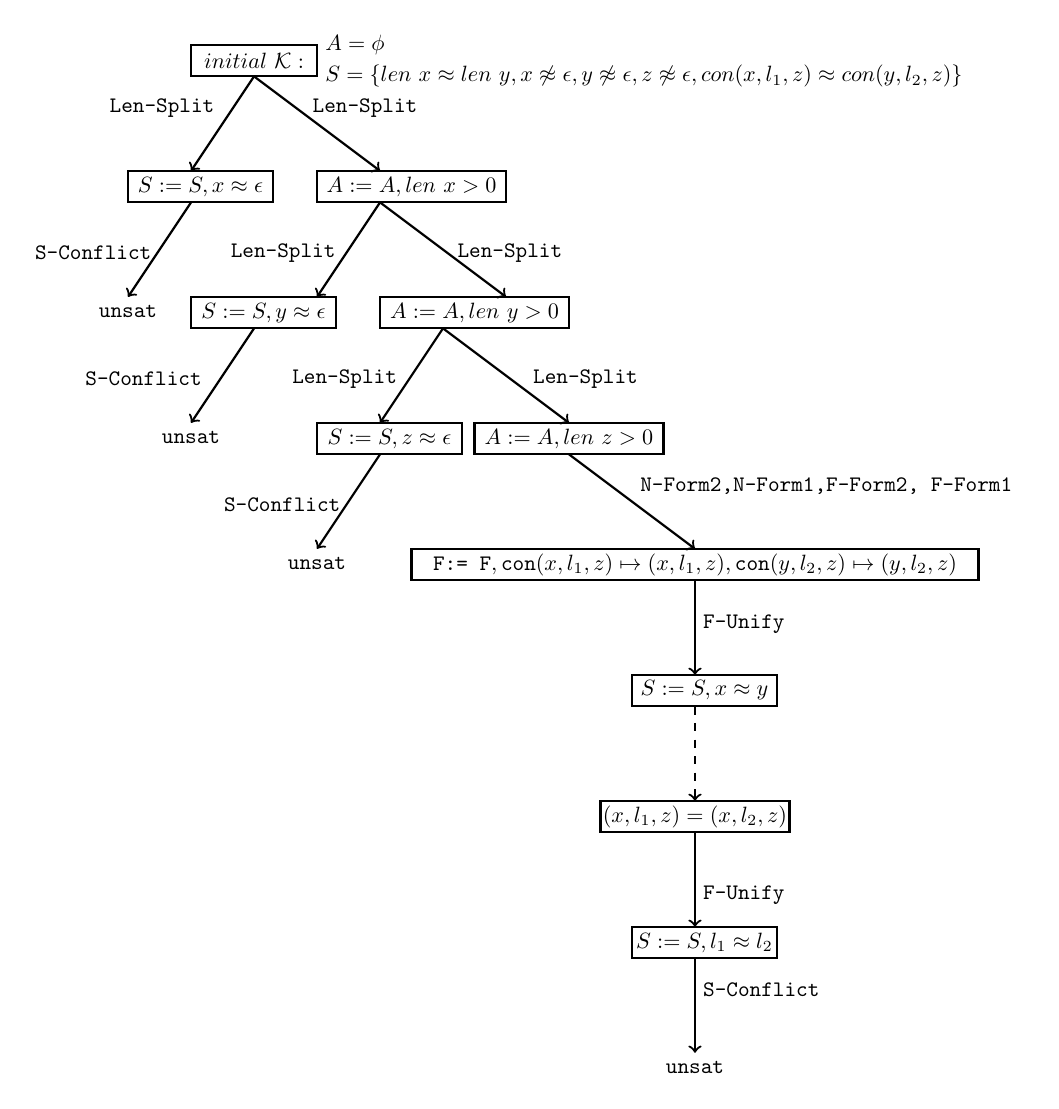
\begin{tikzpicture}[thick,scale=0.8, every node/.style={transform shape}]
	
	\node [right] at (3,20) { $ A=\phi $};
	\node [right] at (3,19.5) { $ S=\{  len \ x \approx len \ y, x \not\approx \epsilon, y \not\approx \epsilon,
		z \not\approx \epsilon, con (x, l_1,z) \approx con (y, l_2, z)\} $}; 
	 
    \draw (1,20) rectangle (3,19.5) node[pos=.5] {$ initial \ \mathcal{K}:$};
	
	\draw [->] (2,19.5) -- (1,18);
	\node [left] at (1.5,19) {$\texttt{Len-Split}$};
	
	\draw [->] (2,19.5) -- (4,18);
	\node [right] at (2.8,19) {$\texttt{Len-Split}$};
	
	
	\draw (0,18) rectangle (2.3,17.5) node[pos=.5] {$S:=S, x\approx \epsilon$};
	\node [rectangle, below] at (1,18) {};
	
	
	\draw (3,18) rectangle (6,17.5) node[pos=.5] {$A:=A, len \ x  > 0$};
	\node [rectangle, below] at (4,18) {};
	
	\draw [->] (1,17.5) -- (0,16);
	\node [left] at (0.5,16.7) {$\texttt{S-Conflict}$};
	
	\draw [->] (4,17.5) -- (3,16);
	\node [right] at (1.5,16.7) {$\texttt{Len-Split}$};
	\draw [->] (4,17.5) -- (6,16);
	\node [right] at (5.1,16.7) {$\texttt{Len-Split}$};
	
	\node [below] at (0,16) {$\texttt{unsat}$};
	\draw (1,16) rectangle (3.3,15.5) node[pos=.5] {$S:=S, y\approx \epsilon$};
	\node [below] at (2,16) {};
	\draw (4,16) rectangle (7,15.5) node[pos=.5] {$A:=A, len \ y  > 0$};
	\node [below] at (5,16) {};
	
	\draw [->] (2,15.5) -- (1,14);
	\node [left] at (1.3,14.7) {$\texttt{S-Conflict}$};
	\draw [->] (5,15.5) -- (4,14);
	\node [left] at (4.4,14.7) {$\texttt{Len-Split}$};	
	\draw [->] (5,15.5) -- (7,14);
	\node [right] at (6.3,14.7) {$\texttt{Len-Split}$};
	
	
	\node [below] at (1,14) {$\texttt{unsat}$};
	\draw (3,14) rectangle (5.3,13.5) node[pos=.5] {$S:=S, z\approx \epsilon$};
	\node [below] at (4,14) {};
	\draw (5.5,14) rectangle (8.5,13.5) node[pos=.5] {$A:=A, len \ z  > 0$};
	\node [below] at (7,14) {};


	\draw [->] (4,13.5) -- (3,12);
	\node [left] at (3.5,12.7) {$\texttt{S-Conflict}$};
	\draw [->] (7,13.5) -- (9,12);
    \node [right] at (8,13) {$\texttt{N-Form2,N-Form1,F-Form2, F-Form1 }$};
    

	
	\node [below] at (3,12) {$\texttt{unsat}$};
	\draw (4.5,12) rectangle (13.5,11.5) node[pos=.5] {$\texttt{F:= F},\texttt{con}(x,l_1,z)\mapsto (x,l_1,z),\texttt{con}(y,l_2,z)\mapsto(y,l_2,z)$};
	\node [below] at (9,12) {};
	
	\draw [->] (9,11.5) -- (9,10);
	\node [right] at (9,10.8) {$\texttt{F-Unify}$};
	
	\draw (8,10) rectangle (10.3,9.5) node[pos=.5] {$S:=S, x\approx y$};
	\node [below] at (9,10) {};
	
	\draw [dashed,->] (9,9.5) -- (9,8);
	
	\draw (7.5,8) rectangle (10.5,7.5) node[pos=.5] {$( x, l_1, z ) = (x, l_2,z)$};
	\node [below] at (9,8) {};
	
	\draw [->] (9,7.5) -- (9,6);
	\node [right] at (9,6.5) {$\texttt{F-Unify}$};
	
	\draw (8,6) rectangle (10.3,5.5) node[pos=.5] {$S:=S, l_1 \approx l_2$};
	\node [below] at (9,6) {};
	
	\draw [->] (9,5.5) -- (9,4);
	\node [right] at (9,5) {$\texttt{S-Conflict}$};
	
	\node [below] at (9,4) {$\texttt{unsat}$};
	
	
	
	
	
	
	\end{tikzpicture}
	\caption{The derivation tree for example 1. Here $l_1, l_2 $ are distinct constants of same length.}
\end{figure}	

    %\begin{figure}
\centering
\begin{tikzpicture}
\draw [lightgray](0,0) --(0,20) -- (15,20)-- (15,0) --(0,0);
\draw [lightgray](0,1) --(15,1);
\draw [lightgray](0,2) --(15,2);
\draw [lightgray](0,3) --(15,3);
\draw [lightgray](0,4) --(15,4);
\draw [lightgray](0,5) --(15,5);
\draw [lightgray](0,6) --(15,6);
\draw [lightgray](0,7) --(15,7);
\draw [lightgray](0,8) --(15,8);
\draw [lightgray](0,9) --(15,9);
\draw [lightgray](0,10) --(15,10);
\draw [lightgray](0,11) --(15,11);
\draw [lightgray](0,12) --(15,12);
\draw [lightgray](0,13) --(15,13);
\draw [lightgray](0,14) --(15,14);
\draw [lightgray](0,15) --(15,15);
\draw [lightgray](0,16) --(15,16);
\draw [lightgray](0,17) --(15,17);
\draw [lightgray](0,18) --(15,18);
\draw [lightgray](0,19) --(15,19);
\draw [lightgray](0,20) --(15,20);

\draw [lightgray](0,7.5) --(7.5,20);

\node [below] at (10,10) {$ initial \ \mathcal{K}$};
\node [below] at (10,9.6) {$\texttt{Len-Split}$};

\draw [->] (10,9.3) -- (8,8.5);
\draw [->] (10,9.3) -- (12,8.5);


\draw [->] (5,5) -- (4,4.5);
\node [right] at (2,8) {$\texttt{F:= F},\texttt{con}(x,l_1,z)\mapsto (x,l_1,z),\texttt{con}(y,l_2,z)\mapsto(y,l_2,z)$};
\node [right] at (6,7.2) {$\texttt{F-Unify}$};
\draw [->] (6,7.8) -- (6,6.8);
\node [right] at (5,6.5) {$\texttt{S:= S},x\approx y$};

\end{tikzpicture}
\caption{The derivation tree for example 1.}
\end{figure}



    \section{Evaluation}
\label{sec:evaluation}
According to the authors \cite{main-paper}, a theory solver based procedure described in the previous sections, is implemented as part of SMT solver CVC4. The string alphabet $\mathcal{A}$ for this implementation is the set of all 256 ASCII characters. An experimental comparison with two other the string solvers was conducted. The other string solvers are Z3-STR \cite{Z3_str} and Kaluza \cite{Kaluza}. These two solvers are widely used in security analysis. For the evaluation, 47,284 benchmark problems from a set of about 50K benchmarks generated by Kudzu \cite{Kudzu} were used. These benchmarks were translated into CVC4’s extension of the SMT-LIB format and into the Z3-STR format. In the paper \cite{main-paper}, it is claimed that, CVC4’s string solver performed better. More detail on the evaluation can be found in \cite{main_phd}.
    \section{Conclusion}
\label{sec:conclusion}
In this paper, we tried to present the overview of a automatic reasoning tool for solving constraints over unbounded strings with length. We have found, the idea of implementing the string solver natively is unique. This approach allowed high interaction with core of CVC4 SMT solver. So the performance is better than others. It also allows any general purpose arithmetic solver be easily integrated. However, the application of the rules is complicated and very hard to implement. it would be better to support a richer language of string constraints that occur often in practice, especially in security applications. Such expressiveness would promote the use of such automatic reasoning tool in commercial software constructions. 
    
	
	\newpage
	%Sets the bibliography style to UNSRT and imports the 
	%bibliography file "samples.bib".
	\bibliographystyle{unsrt}
	\bibliography{sample}
	
\end{document}

